

\documentclass[11pt, a4paper]{letter} % Set the font size (10pt, 11pt and 12pt) and paper size (letterpaper, a4paper, etc)

\usepackage{graphicx}
\usepackage{tikz}
\usetikzlibrary{calc}
\usepackage[T1]{fontenc} 
\usepackage[utf8]{inputenc}  
\usepackage{gfsdidot}
\usepackage{microtype}

\pagestyle{empty} 


\setlength\parindent{1cm} 

\newenvironment{myfont}{\fontfamily{pnc}\selectfont}{\par}

\makeatletter
\newcommand{\vhrulefill}[1]{\leavevmode\leaders\hrule\@height#1\hfill \kern\z@}
\makeatother

\usepackage[top=0.5cm, 
bottom=0.5cm, 
left=3cm, 
right=3cm,]{geometry} 
%%%%%%%%%%%%%%%%%%%%%%%%%%%%%%%%%%%%%%%%%
% Based on a Template by
% Brian Moses
% Vel (vel@LaTeXTemplates.com)
%
% License:
% CC BY-NC-SA 3.0 (http://creativecommons.org/licenses/by-nc-sa/3.0/)
%
% This template is only based on the mentioned template and it is not 
% completely the same. 
%%%%%%%%%%%%%%%%%%%%%%%%%%%%%%%%%%%%%%%%%






\newcommand{\Title}[1]{\renewcommand{\Title}{#1}}
\newcommand{\headerlineone}[1]{\renewcommand{\headerlineone}{#1}}
\newcommand{\headerlinetwo}[1]{\renewcommand{\headerlinetwo}{#1}}
\newcommand{\authordetails}[1]{\renewcommand{\authordetails}{#1}}


\address{
	
\includegraphics[width=1in]{sharif1.jpg} 
	\hspace{0.82\textwidth}
	\vskip -0.1\textheight~\\ 
	\Large\hspace{0.2\textwidth}\headerlineone\hfill ~\\[0.006\textheight] 
	\hspace{0.2\textwidth}\headerlinetwo\hfill \normalsize 
	~\\[-0.01\textheight]
	\hspace{0.2\textwidth}\vhrulefill{1pt} \\ 
{
	\hspace{\fill} 
	\parbox[t]{0.48\textwidth}{ 
		\footnotesize 
		{\authordetails}
		\today
	}
}
	\hspace{-0.25\textwidth}
	\vspace{-0.1\textheight} 
}



\renewcommand{\opening}[1]{
	{\centering\fromaddress\vspace{0.05\textheight} \\ }
	{\raggedright \toname \\ \toaddress \par}  
	\vspace{1cm} 
	\noindent #1
}


 
\authordetails{Iman Mohammadi\\
	35 Payambaran St.\\ 
	Tehran \\
	14717-84876\\
	Iran\\ 
}


\headerlineone{Sharif} 

\headerlinetwo{University of Technology}

\begin{document}
	



\begin{letter}{
	Dr. Fazli\\
	Room 818\\
	Department of Computer Engineering\\
	Sharif University of Technology\\
	Azadi Ave\\
	Tehran\\
	11155-1639\\
	Iran
}




\opening{
	\begin{center}
		\begin{myfont}
		\textbf{REQUEST FOR TEACHING ASSISTANT  APPLICATION}
	\end{myfont}
	\end{center}
	Dear Dr. Fazli,}

\begin{flushleft}
I would like to apply for the teaching assistant position in the "Game Theory" course. I have a passion for helping in the teaching process of this subject to the students.

I have taken the course in the fall 2022 semester and had been in the teaching team of the same course instructed by Dr. Nilipour last semester and had helped with the homework. I could utilize my experience from the previous semester to enrich this course.

Thank you for your consideration. I am looking forward to hearing from you in the near future for the course details.



Yours Sincerely,

\hspace*{-0.90cm}
\vspace*{-0.50cm}
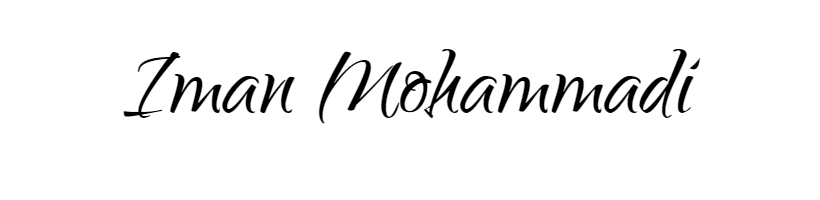
\includegraphics[width = 0.35\textwidth]{sign.png}

Iman Mohammadi
\end{flushleft}


\begin{tikzpicture}[overlay,remember picture]
	\draw [line width=1pt, rounded corners=1pt,]
	($ (current page.north west) + (0.25cm,-0.25cm) $)
	rectangle
	($ (current page.south east) + (-0.25cm,0.25cm) $);       
\end{tikzpicture}
\end{letter}

\end{document}
